\documentclass{article}
% Pre-amble
\usepackage{tikz}
\usepackage[margin=0.5in]{geometry}
\usetikzlibrary{shapes.geometric, arrows}
% Custom Colors
\definecolor{tabblue}{RGB}{31,119,180}
\definecolor{tabor}{RGB}{255,127,14}
\definecolor{tabgreen}{RGB}{44,160,44}
\definecolor{tabred}{RGB}{214,39,40}
\definecolor{tabpur}{RGB}{148,103,189}
\tikzstyle{general} = [rectangle, rounded corners, minimum width=3cm, minimum height=1cm,text centered, draw=black, fill=tabblue!50]
\tikzstyle{decision} = [diamond, minimum width=3cm, minimum height=1cm, text centered, draw=black, fill=tabor!30]
\tikzstyle{result} = [rectangle, rounded corners, minimum width=3cm, minimum height=1cm,text centered, draw=black, fill=tabred!50]
\tikzstyle{arrow} = [thick,->,>=stealth]
\begin{document}
\begin{center}
 \textbf{Overview}\par\medskip
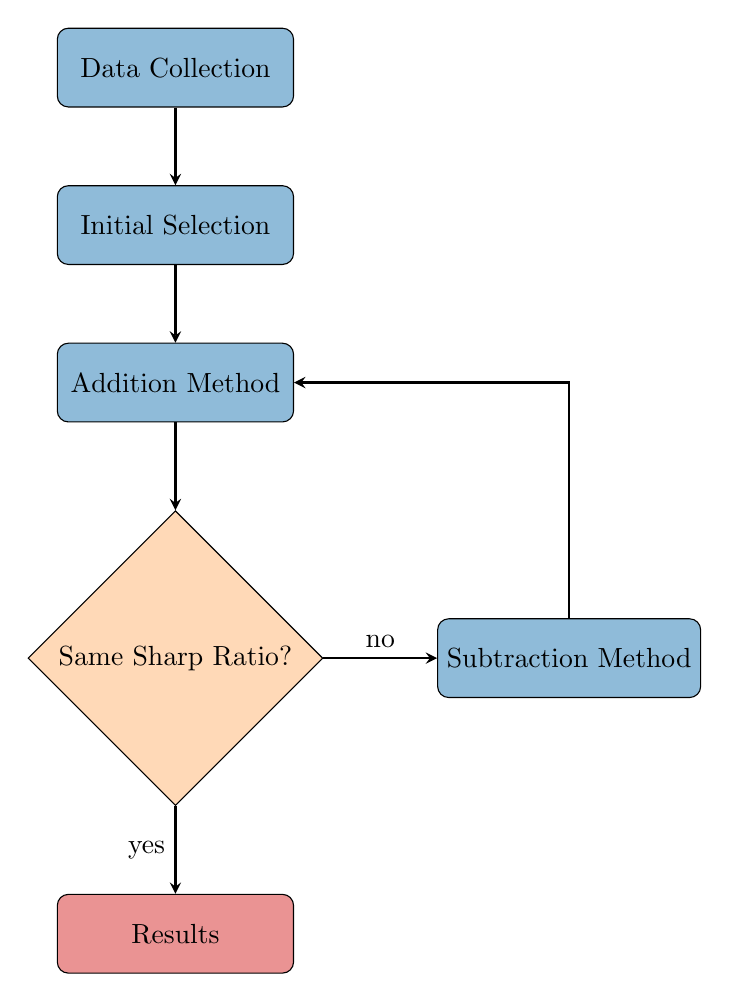
\begin{tikzpicture}
[node distance=2cm]

\node (data) [general] {Data Collection};
\node (select) [general, below of =data] {Initial Selection};
\node (add) [general, below of = select] {Addition Method};
\node (sharpe) [decision, below of = add, yshift = -1.5cm ] {Same Sharp Ratio?};
\node (subtract) [general, right of = sharpe, xshift = 3 cm] {Subtraction Method};
\node(result) [result, below of = sharpe, yshift = -1.5 cm] {Results};

\draw [arrow] (data) -- (select);
\draw [arrow] (select) -- (add);
\draw [arrow] (add) -- (sharpe);
\draw [arrow] (sharpe) -- node[anchor=south] {no} (subtract);
\draw [arrow] (subtract) |- (add);
\draw[arrow] (sharpe) --  node[anchor=east] {yes} (result);

\end{tikzpicture}
\end{center}


\begin{center}
\textbf{Addition Method}\par\medskip
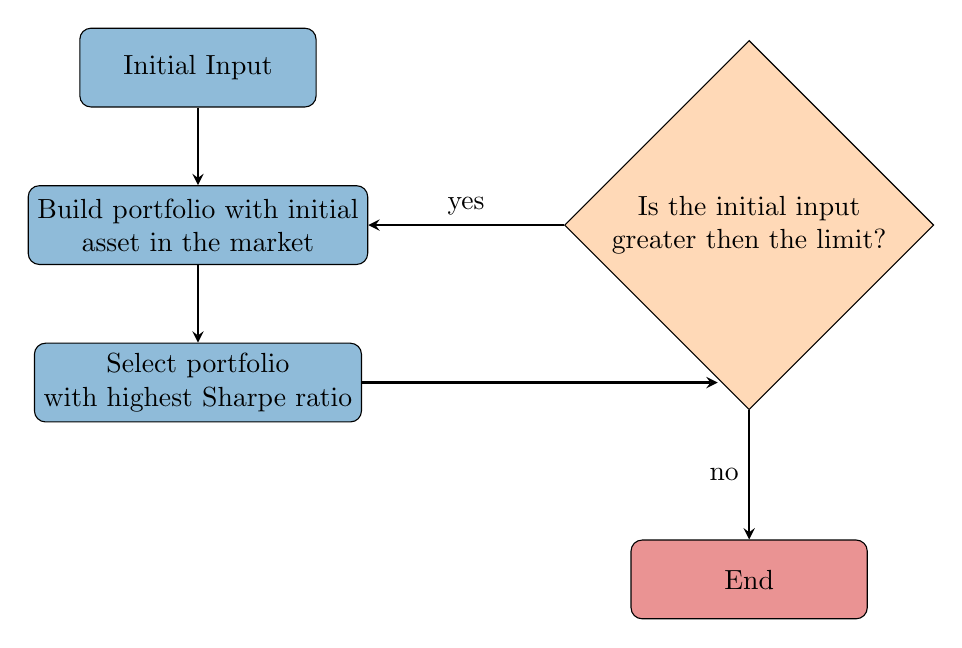
\begin{tikzpicture}
[node distance=2cm, nodes = {align = center},]

\node (input) [general] {Initial Input};
\node (build) [general,below of = input,align=center] {Build portfolio with initial \\asset in the market};
\node (select1) [general,below of = build,align=center] {Select portfolio \\with highest Sharpe ratio};
\node (greater) [decision, right of = build,align=center, xshift = 5cm] {Is the initial input \\ greater then the limit?};
\node(end) [result, below of = greater,yshift = -2.5cm] {End};

\draw [arrow] (input) -- (build);
\draw [arrow] (build) -- (select1);
\draw [arrow] (select1) -- ++(6.6,0)(greater);
\draw [arrow] (greater) -- node[anchor=east] {no} (end);
\draw [arrow] (greater) -- node[anchor=south] {yes} (build);
\end{tikzpicture}
\end{center}
\newpage
\begin{center}
\textbf{Reduction Method}\par\medskip
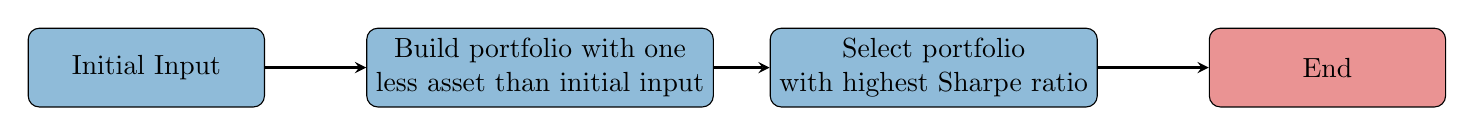
\begin{tikzpicture}
[node distance=5cm]

\node (input) [general] {Initial Input};
\node (build) [general,right of = input,align=center] {Build portfolio with one \\less asset than initial input};
\node (select) [general,right of = build,align=center] {Select portfolio \\with highest Sharpe ratio};
\node(end) [result, right of  = select] {End};

\draw [arrow] (input) -- (build);
\draw [arrow] (build) -- (select);
\draw [arrow] (select) -- (end);

\end{tikzpicture}
\end{center}

\begin{center}
\textbf{Quasi Bisection}\par\medskip
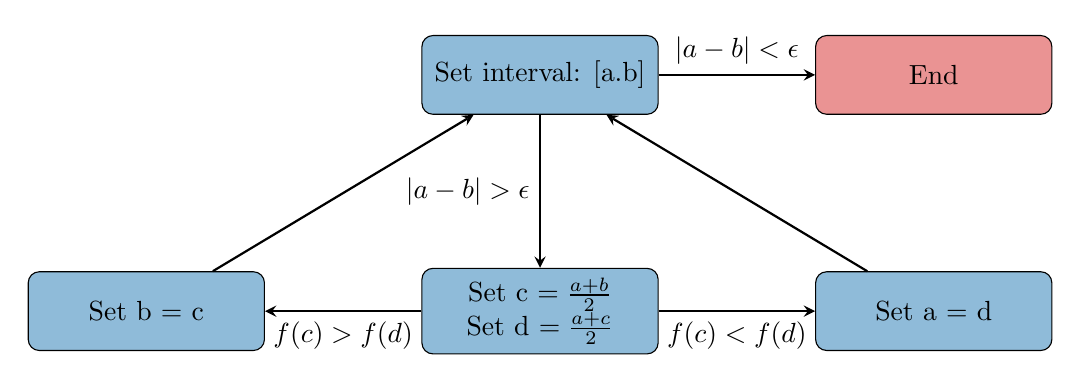
\begin{tikzpicture}
[node distance=5cm,nodes={align=center}]
\node (interval) [general] {Set interval: [a.b]};
\node (done) [result,right of = interval,align=center] {End};
\node (set) [general,below of = interval,align = center,yshift = 2cm] {Set c $= \frac{a+b}{2}$\\Set d $= \frac{a+c}{2}$};
\node (ad) [general, right of = set] {Set a = d};
\node (bc) [general, left of = set] {Set b = c};


\draw [arrow] (interval) -- node[anchor=south] {$|a-b|<\epsilon$}(done);
\draw [arrow] (interval) -- node[anchor=east] {$|a-b|>\epsilon$}(set);
\draw [arrow] (set) -- node[anchor=north] {$f(c)<f(d)$}(ad);
\draw [arrow] (set) -- node[anchor=north] {$f(c)>f(d)$}(bc);
\draw [arrow] (ad) -- (interval);
\draw [arrow] (bc) -- (interval);

\end{tikzpicture}
\end{center}


\end{document}